% Options for packages loaded elsewhere
\PassOptionsToPackage{unicode}{hyperref}
\PassOptionsToPackage{hyphens}{url}
\PassOptionsToPackage{dvipsnames,svgnames,x11names}{xcolor}
%
\documentclass[
  letterpaper,
  DIV=11,
  numbers=noendperiod]{scrartcl}

\usepackage{amsmath,amssymb}
\usepackage{iftex}
\ifPDFTeX
  \usepackage[T1]{fontenc}
  \usepackage[utf8]{inputenc}
  \usepackage{textcomp} % provide euro and other symbols
\else % if luatex or xetex
  \usepackage{unicode-math}
  \defaultfontfeatures{Scale=MatchLowercase}
  \defaultfontfeatures[\rmfamily]{Ligatures=TeX,Scale=1}
\fi
\usepackage{lmodern}
\ifPDFTeX\else  
    % xetex/luatex font selection
\fi
% Use upquote if available, for straight quotes in verbatim environments
\IfFileExists{upquote.sty}{\usepackage{upquote}}{}
\IfFileExists{microtype.sty}{% use microtype if available
  \usepackage[]{microtype}
  \UseMicrotypeSet[protrusion]{basicmath} % disable protrusion for tt fonts
}{}
\makeatletter
\@ifundefined{KOMAClassName}{% if non-KOMA class
  \IfFileExists{parskip.sty}{%
    \usepackage{parskip}
  }{% else
    \setlength{\parindent}{0pt}
    \setlength{\parskip}{6pt plus 2pt minus 1pt}}
}{% if KOMA class
  \KOMAoptions{parskip=half}}
\makeatother
\usepackage{xcolor}
\setlength{\emergencystretch}{3em} % prevent overfull lines
\setcounter{secnumdepth}{5}
% Make \paragraph and \subparagraph free-standing
\makeatletter
\ifx\paragraph\undefined\else
  \let\oldparagraph\paragraph
  \renewcommand{\paragraph}{
    \@ifstar
      \xxxParagraphStar
      \xxxParagraphNoStar
  }
  \newcommand{\xxxParagraphStar}[1]{\oldparagraph*{#1}\mbox{}}
  \newcommand{\xxxParagraphNoStar}[1]{\oldparagraph{#1}\mbox{}}
\fi
\ifx\subparagraph\undefined\else
  \let\oldsubparagraph\subparagraph
  \renewcommand{\subparagraph}{
    \@ifstar
      \xxxSubParagraphStar
      \xxxSubParagraphNoStar
  }
  \newcommand{\xxxSubParagraphStar}[1]{\oldsubparagraph*{#1}\mbox{}}
  \newcommand{\xxxSubParagraphNoStar}[1]{\oldsubparagraph{#1}\mbox{}}
\fi
\makeatother


\providecommand{\tightlist}{%
  \setlength{\itemsep}{0pt}\setlength{\parskip}{0pt}}\usepackage{longtable,booktabs,array}
\usepackage{calc} % for calculating minipage widths
% Correct order of tables after \paragraph or \subparagraph
\usepackage{etoolbox}
\makeatletter
\patchcmd\longtable{\par}{\if@noskipsec\mbox{}\fi\par}{}{}
\makeatother
% Allow footnotes in longtable head/foot
\IfFileExists{footnotehyper.sty}{\usepackage{footnotehyper}}{\usepackage{footnote}}
\makesavenoteenv{longtable}
\usepackage{graphicx}
\makeatletter
\def\maxwidth{\ifdim\Gin@nat@width>\linewidth\linewidth\else\Gin@nat@width\fi}
\def\maxheight{\ifdim\Gin@nat@height>\textheight\textheight\else\Gin@nat@height\fi}
\makeatother
% Scale images if necessary, so that they will not overflow the page
% margins by default, and it is still possible to overwrite the defaults
% using explicit options in \includegraphics[width, height, ...]{}
\setkeys{Gin}{width=\maxwidth,height=\maxheight,keepaspectratio}
% Set default figure placement to htbp
\makeatletter
\def\fps@figure{htbp}
\makeatother
% definitions for citeproc citations
\NewDocumentCommand\citeproctext{}{}
\NewDocumentCommand\citeproc{mm}{%
  \begingroup\def\citeproctext{#2}\cite{#1}\endgroup}
\makeatletter
 % allow citations to break across lines
 \let\@cite@ofmt\@firstofone
 % avoid brackets around text for \cite:
 \def\@biblabel#1{}
 \def\@cite#1#2{{#1\if@tempswa , #2\fi}}
\makeatother
\newlength{\cslhangindent}
\setlength{\cslhangindent}{1.5em}
\newlength{\csllabelwidth}
\setlength{\csllabelwidth}{3em}
\newenvironment{CSLReferences}[2] % #1 hanging-indent, #2 entry-spacing
 {\begin{list}{}{%
  \setlength{\itemindent}{0pt}
  \setlength{\leftmargin}{0pt}
  \setlength{\parsep}{0pt}
  % turn on hanging indent if param 1 is 1
  \ifodd #1
   \setlength{\leftmargin}{\cslhangindent}
   \setlength{\itemindent}{-1\cslhangindent}
  \fi
  % set entry spacing
  \setlength{\itemsep}{#2\baselineskip}}}
 {\end{list}}
\usepackage{calc}
\newcommand{\CSLBlock}[1]{\hfill\break\parbox[t]{\linewidth}{\strut\ignorespaces#1\strut}}
\newcommand{\CSLLeftMargin}[1]{\parbox[t]{\csllabelwidth}{\strut#1\strut}}
\newcommand{\CSLRightInline}[1]{\parbox[t]{\linewidth - \csllabelwidth}{\strut#1\strut}}
\newcommand{\CSLIndent}[1]{\hspace{\cslhangindent}#1}

\KOMAoption{captions}{tableheading}
\makeatletter
\@ifpackageloaded{caption}{}{\usepackage{caption}}
\AtBeginDocument{%
\ifdefined\contentsname
  \renewcommand*\contentsname{Table of contents}
\else
  \newcommand\contentsname{Table of contents}
\fi
\ifdefined\listfigurename
  \renewcommand*\listfigurename{List of Figures}
\else
  \newcommand\listfigurename{List of Figures}
\fi
\ifdefined\listtablename
  \renewcommand*\listtablename{List of Tables}
\else
  \newcommand\listtablename{List of Tables}
\fi
\ifdefined\figurename
  \renewcommand*\figurename{Figure}
\else
  \newcommand\figurename{Figure}
\fi
\ifdefined\tablename
  \renewcommand*\tablename{Table}
\else
  \newcommand\tablename{Table}
\fi
}
\@ifpackageloaded{float}{}{\usepackage{float}}
\floatstyle{ruled}
\@ifundefined{c@chapter}{\newfloat{codelisting}{h}{lop}}{\newfloat{codelisting}{h}{lop}[chapter]}
\floatname{codelisting}{Listing}
\newcommand*\listoflistings{\listof{codelisting}{List of Listings}}
\makeatother
\makeatletter
\makeatother
\makeatletter
\@ifpackageloaded{caption}{}{\usepackage{caption}}
\@ifpackageloaded{subcaption}{}{\usepackage{subcaption}}
\makeatother

\ifLuaTeX
  \usepackage{selnolig}  % disable illegal ligatures
\fi
\usepackage{bookmark}

\IfFileExists{xurl.sty}{\usepackage{xurl}}{} % add URL line breaks if available
\urlstyle{same} % disable monospaced font for URLs
\hypersetup{
  pdftitle={Uncovering Ferry Traffic Patterns: A Data-Driven Study of Toronto Island Ticket Sales and Redemptions},
  pdfauthor={Yingke He},
  colorlinks=true,
  linkcolor={blue},
  filecolor={Maroon},
  citecolor={Blue},
  urlcolor={Blue},
  pdfcreator={LaTeX via pandoc}}


\title{Uncovering Ferry Traffic Patterns: A Data-Driven Study of Toronto
Island Ticket Sales and Redemptions\thanks{Code and data are available
at: https://github.com/ohyykk/ferrySale.git}}
\author{Yingke He}
\date{September 23, 2024}

\begin{document}
\maketitle
\begin{abstract}
This study examines the ticket redemption and sales counts for the
Toronto Island Ferry, analyzing time-based trends and the relationships
between sales and redemptions. Statistical models are developed to
predict ferry ticket usage. The results uncover seasonal trends,
operational inefficiencies, and discrepancies between ticket sales and
redemptions, highlighting the need for improved resource management and
service adjustments to better align with fluctuating passenger demand.
These findings offer insights into usage patterns, operational
considerations, and suggest avenues for future research, particularly in
optimizing ticketing strategies and resource allocation.
\end{abstract}

\renewcommand*\contentsname{Table of contents}
{
\hypersetup{linkcolor=}
\setcounter{tocdepth}{3}
\tableofcontents
}

\section{Introduction}\label{introduction}

The Toronto Island Ferry system has long been an essential
transportation link between downtown Toronto and the Toronto Islands,
serving both residents and tourists. With roots tracing back to the
early days of the city's development, the ferry system reflects both
historical and contemporary mobility patterns in the region. Historical
accounts provided by Varga (1987) highlight the evolution of the Toronto
Islands' natural environment and its significance to the area's
biodiversity and recreation. Additionally, the potential role of ferries
in urban transit systems, as explained by Kopystynski (1979), shows
their importance in enhancing urban mobility and connectivity.

With the ticket counts for the Toronto Island Ferry and the trends in
ticket redemption and sales, we can find the connections between
historical developments and current usage patterns. By combining both
historical and modern perspectives and including contemporary studies on
ferry commuting from Roseman (2020), the analysis provides a
comprehensive understanding of the factors influencing ferry usage.
Statistical models are used to analyze ferry ticket demand while showing
the seasonal fluctuations and operational challenges.

Despite the longstanding role of the Toronto Island Ferry system in
connecting downtown Toronto with the Toronto Islands, there is limited
research on the detailed patterns of ferry usage and the efficiency of
the service. While the ferry system serves both residents and tourists,
the lack of data-driven analysis makes it harder to optimize ferry
operations, manage peak demand periods, and improve ticketing
strategies. It is important to fill this gap because of the ferry's dual
function of accommodating daily commuters alongside a significant influx
of seasonal visitors, which introduces variability in service demand.
Without a comprehensive understanding of the underlying trends in ticket
sales and redemptions, it becomes challenging to address inefficiencies
or anticipate future operational challenges. We will address this
problem by providing a detailed analysis of ticketing patterns and
offering insights into how the ferry system can better meet passenger
needs through data-informed decision-making.

In addition to the expected peaks during high tourism periods, this
study investigates inconsistencies between tickets sold and redeemed,
offering insights into potential service inefficiencies. The dual role
of the Toronto Island Ferry system in accommodating both daily commuters
and a large number of seasonal visitors makes it an important case study
in urban transportation planning.

The remainder of this paper is structured as follows:
Section~\ref{sec-data} introduces the dataset used for the analysis,
explaining the key variables and presenting key data analysis.
Section~\ref{sec-discussion} discusses the implications of the findings
and potential directions for future research. Additional information is
presented in the appendix at Section~\ref{sec-appendix}. R Core Team
(2023) and Wickham et al. (2019a) is utilized for the coding proposes of
this paper, and the data section is referenced using
Section~\ref{sec-data}.

\section{Data}\label{sec-data}

\subsection{Overview}\label{sec-data-overview}

The dataset used in this analysis is the 2024 installment of ``Toronto
Island Ferry Ticket Counts'' obtained from OpenDataToronto (Varga
(1987)). This dataset contains information about the number of ferry
tickets redeemed and sold for the Toronto Island Ferry system, which
serves as a critical transportation link between downtown Toronto and
the Toronto Islands.

The dataset is updated regularly and includes time-stamped entries for
ticket redemptions and sales, allowing for a detailed analysis of ferry
usage patterns throughout the year. The data is considered ``open data''
and can be utilized for various analytical purposes, provided that
appropriate attribution is given..

The primary variables included in this analysis are:

\textbf{Timestamp}: The date and time when each ticket count was
recorded.\\
\textbf{Redemption.Count}: The number of ferry tickets redeemed during
the specified time period.\\
\textbf{Sales.Count}: The number of ferry tickets sold during the
specified time period.

The data was processed and analyzed using the R programming language (R
Core Team (2023)). The tidyverse (Wickham et al. (2019b)) and
opendatatoronto packages were employed to download, clean, and prepare
the dataset for analysis. The resulting cleaned dataset was then
utilized to generate the visualizations and statistical analyses
presented in this paper using a collection of libraries which included
the following packages:

\begin{itemize}
\tightlist
\item
  ggplot2 (Wickham 2016)
\item
  knitr (Xie 2023)
\item
  readr (Wickham, Hester, and Bryan 2023)
\end{itemize}

\subsection{Measurements}\label{measurements}

This report utilizes the Toronto Island Ferry Ticket Counts dataset
published by the City of Toronto on the Open Data Portal(City of Toronto
(2024)). Specifically, time-stamped records of both ticket sales and
redemptions were recoreded. Every time a ticket is sold or redeemed, it
represents a physical action by a ferry passenger in Toronto traveling
to the Toronto Island. Actions are then recorded by the ticketing
systems, which automatically records the transaction timestamp, along
with the number of tickets sold and redeemed at that specific time.

This process converts individual passenger transactions into structured
dataset entries, with timestamps to enable tracking over time. The data
captures real-world trends such as higher ferry activity during peak
tourism seasons or weekends, providing useful insights into ferry usage
patterns. It enables further research to analyze passenger demand and
operational trends, helping to make more effective ferry management
decisions.

\subsection{Results}\label{sec-data-resultsk}

Table~\ref{tbl-cleaned_data} provides a detailed snapshot of the Toronto
Island Ferry ticket transactions for a specific time period. It includes
a unique ID for each transaction, the Time at which each transaction
occurred, the number of Tickets Redeemed, the number of Tickets Sold,
and the Date of the transaction.

\begin{longtable}[]{@{}ccccc@{}}

\caption{\label{tbl-cleaned_data}Sample of cleaned Ferry Ticket Counts
Data}

\tabularnewline

\toprule\noalign{}
ID & Time & Tickets Redeemed & Tickets Sold & Date \\
\midrule\noalign{}
\endhead
\bottomrule\noalign{}
\endlastfoot
51 & 23:30:00 & 5 & 4 & 2024-09-24 \\
52 & 23:15:00 & 1 & 3 & 2024-09-24 \\
53 & 23:00:00 & 2 & 0 & 2024-09-24 \\
54 & 22:45:00 & 7 & 3 & 2024-09-24 \\
55 & 22:30:00 & 11 & 0 & 2024-09-24 \\
56 & 22:15:00 & 2 & 1 & 2024-09-24 \\
57 & 22:00:00 & 5 & 6 & 2024-09-24 \\
58 & 21:45:00 & 2 & 3 & 2024-09-24 \\
59 & 21:30:00 & 14 & 41 & 2024-09-24 \\
60 & 21:15:00 & 3 & 1 & 2024-09-24 \\

\end{longtable}

The above table shows the typical flucuations in ticket sales and
redemptions throughout the day. For example, during late evening hours,
we observe varying ticket redemption and sales patterns, which may
correspond to changes in passenger demand as the ferry service
approaches the end of its operational hours.

\begin{longtable}[]{@{}ccccc@{}}
\caption{Summary Statistics of Ticket
Counts}\label{tbl-summary_stats}\tabularnewline
\toprule\noalign{}
Avg Redeemed & Avg Sold & Max Redeemed & Max Sold & Count \\
\midrule\noalign{}
\endfirsthead
\toprule\noalign{}
Avg Redeemed & Avg Sold & Max Redeemed & Max Sold & Count \\
\midrule\noalign{}
\endhead
\bottomrule\noalign{}
\endlastfoot
48.44548 & 49.36013 & 7216 & 7229 & 229380 \\
\end{longtable}

The summary statistics, shown in Table~\ref{tbl-summary_stats}, provide
a clear understanding of ferry ticket trends. The high volume of tickets
sold and redeemed indicates strong demand for the ferry service, with
the close alignment between sales and redemptions suggesting high
customer engagement. On average, 46.36 tickets were sold every 15
minutes during working hours, and 48.45 tickets were redeemed,
highlighting that most customers have used their tickets. The small gap
between sales and redemptions implies a few no-shows or unused tickets.
The maximum values of 7,216 for sales and 7,229 for redemptions
demonstrate the ferry's capacity to handle high passenger volumes,
typically operating at full capacity on busy days.

\subsubsection{Temporal Trends in Redemption and Sales
Counts}\label{sec-data-temporal}

To gain an initial insight into the dataset, we plotted the trends in
ticket redemption and sales counts over time. The line plot shown in
Figure~\ref{fig-linePlot1}, Figure~\ref{fig-linePlot2},
Figure~\ref{fig-linePlot3} and Figure~\ref{fig-linePlot4} provides a
clear visual representation of these trends, serving as a starting point
for deeper analysis of ferry usage patterns.

The peak day analysis table below highlights the highest ferry ticket
sales, often aligning with public holidays or major events, such as Aug
1 2016, and July 1 2018. On September 15, 2020, ferry sales saw a
significant drop, with only 5,003 tickets sold. This decline could be
due to the impact of COVID-19(Lee and Leung (2021)).

\begin{longtable}[]{@{}rlr@{}}
\caption{Table: Peak Day for Each Year Based on Total
Sales}\tabularnewline
\toprule\noalign{}
Year & Peak Day & Total Sales \\
\midrule\noalign{}
\endfirsthead
\toprule\noalign{}
Year & Peak Day & Total Sales \\
\midrule\noalign{}
\endhead
\bottomrule\noalign{}
\endlastfoot
2015 & 2015-07-18 & 23354 \\
2016 & 2016-08-01 & 25552 \\
2017 & 2017-08-20 & 17322 \\
2018 & 2018-07-01 & 23669 \\
2019 & 2019-08-04 & 20911 \\
2020 & 2020-09-05 & 5003 \\
2021 & 2021-09-05 & 12356 \\
2022 & 2022-07-16 & 20419 \\
2023 & 2023-08-19 & 20203 \\
2024 & 2024-07-13 & 19603 \\
\end{longtable}

The dataset used in this analysis provides timestamped records of ticket
redemptions and sales for the Toronto Island Ferry system, allowing for
a detailed time series analysis of ferry usage patterns. As illustrated
in Figure~\ref{fig-linePlot1}, ferry usage fluctuates significantly
throughout the year, with peak activity consistently observed between
July and September. This pattern corresponds to the increased passenger
demand during the summer holiday season and major events. In 2020,
ticket demand saw a sharp decline, likely due to the impact of the
COVID-19 pandemic(Urbanyi-Popiolek (2020)), but it showed signs of
gradual recovery starting in 2021 as restrictions eased and tourism
began to rebound in Toronto(Government of Canada (2024)). By identifying
these peak traffic periods in advance, ferry operators can implement
targeted operational strategies, such as scheduling additional ferry
trips or introducing crowd control measures to minimize the risk of
overcrowding or service disruptions. Identifing these high-demand
periods can ensure smoother ferry operations and enhance the overall
passenger experience.

\begin{figure}

\centering{

\includegraphics{paper_files/figure-pdf/fig-linePlot1-1.pdf}

}

\caption{\label{fig-linePlot1}Redemption and Sales Counts Over Time in
days}

\end{figure}%

加一小段描述描述figure1

Figure~\ref{fig-linePlot2} below shows the Redemption and Sales Counts
in months over years, 加一段描述figure2

\newpage

\begin{figure}[H]

\centering{

\includegraphics{paper_files/figure-pdf/fig-linePlot2-1.pdf}

}

\caption{\label{fig-linePlot2}Redemption and Sales Counts Over Time in
months}

\end{figure}%

Figure~\ref{fig-linePlot3} on the next page compares the sales count and
redemption count in year 2021 and 2023

1 emm这里写一点描述fig3的对比?,render后看页面排版

\begin{figure}[H]

\centering{

\includegraphics{paper_files/figure-pdf/fig-linePlot3-1.pdf}

}

\caption{\label{fig-linePlot3}Redemption and Sales Counts Over Time in
2021 and 2023}

\end{figure}%

As shown in Figure~\ref{fig-linePlot4}, the x-axis denotes the
timestamps of each record, while the y-axis represents the number of
tickets processed. The blue line corresponds to the redemption counts,
and the green line represents the sales counts, plotted inversely to
emphasize the contrast between the two trends. The symmetrical y-axis
allows for a clearer comparison between peaks and troughs in both counts
over time.

\begin{figure}[H]

\centering{

\includegraphics{paper_files/figure-pdf/fig-linePlot4-1.pdf}

}

\caption{\label{fig-linePlot4}Redemption and Sales Counts Over Time in
years}

\end{figure}%

The plot reveals significant variations in ferry usage over years. We
observe several peaks in both redemption and sales counts, likely
aligning with periods of high activity, such as weekends, holidays, or
the peak tourist season during the summer months. These spikes suggest
increased demand during favorable weather or event-driven occasions.
Conversely, the noticeable dips in the graph may correspond to regular
weekdays or off-season times, indicating lower ferry usage during these
periods. This information is valuable for understanding the temporal
dynamics of ferry operations and can inform better resource management
and scheduling.

\subsubsection{Comparative Analysis of Ticket Sales and
Redemptions}\label{comparative-analysis-of-ticket-sales-and-redemptions}

The scatter plot in Figure~\ref{fig-scatterPlot} is designed to explore
the relationship between ticket redemption and sales counts for the
Toronto Island Ferry system. This visualization allows us to understand
whether there is a correlation between the number of tickets sold and
the number of tickets redeemed during the same time period.

\begin{figure}

\centering{

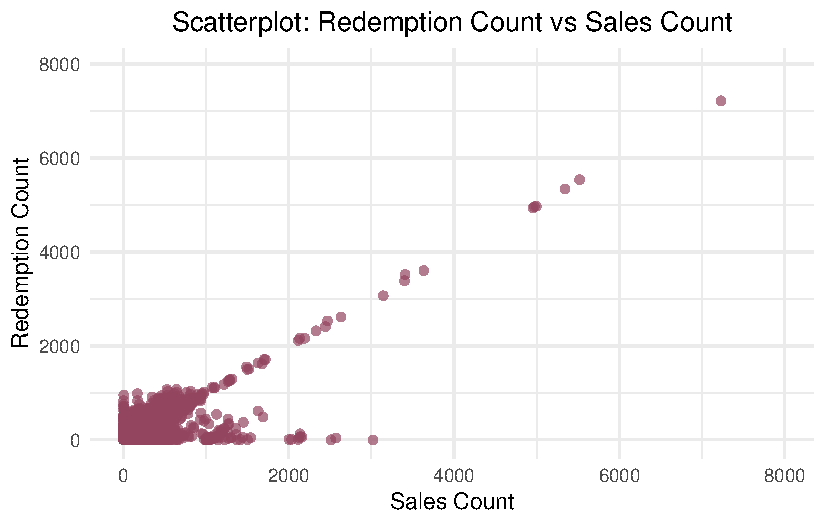
\includegraphics{paper_files/figure-pdf/fig-scatterPlot-1.pdf}

}

\caption{\label{fig-scatterPlot}Scatter Plot of Redemption vs Sales
Count}

\end{figure}%

Figure~\ref{fig-scatterPlot} displays each data point as a purple dot,
where the y-axis represents the count of tickets redeemed, and the
x-axis denotes the count of tickets sold. This plot provides insight
into the degree of alignment between ticket sales and actual usage
(redemptions).

The scatter plot shows how ticket sales and redemptions relate to each
other over time. If most points lie along a diagonal line, it indicates
a strong positive correlation between the two variables, suggesting that
a high number of tickets sold typically corresponds to a high number of
tickets redeemed. This scenario could imply effective ticket
utilization, where most purchased tickets are being used for travel.

\subsubsection{Visual Comparison of Ticket Sales and Redemption
Distribution}\label{visual-comparison-of-ticket-sales-and-redemption-distribution}

The box plot shown in Figure~\ref{fig-boxPlot} provides a summary of the
distribution of ticket sales and redemption counts for the Toronto
Island Ferry system. This visualization helps to identify the spread,
central tendency, and any potential outliers in the data for both
categories, offering a comparative view of the sales and redemption
behaviors.

\begin{figure}

\centering{

\includegraphics{paper_files/figure-pdf/fig-boxPlot-1.pdf}

}

\caption{\label{fig-boxPlot}Box Plot of Sales and Redemption Counts}

\end{figure}%

Figure~\ref{fig-boxPlot} illustrates two box plots side by side: one for
sales counts (light blue) and the other for redemption counts (light
green). Each box plot provides a visual summary of the data
distribution, highlighting the median, quartiles, and any outliers for
each category.

The box plots reveal key differences and similarities in the
distribution of sales and redemption counts. The horizontal line inside
each box represents the median count, providing a measure of central
tendency. The top and bottom edges of the box denote the interquartile
range (IQR), which captures the middle 50\% of the data. The
``whiskers'' extending from the box show the range of values within 1.5
times the IQR from the first and third quartiles, while any points
beyond these whiskers are considered outliers.

\section{Discussion}\label{sec-discussion}

In Section~\ref{sec-data-temporal}, the time series analysis of ticket
sales and redemptions (Figure Figure~\ref{fig-linePlot1},
Figure~\ref{fig-linePlot2}, Figure~\ref{fig-linePlot3} and
Figure~\ref{fig-linePlot4} ) revealed clear seasonal patterns, with
pronounced peaks during the warmer months. This trend aligns with the
historical and cultural significance of the Toronto Islands as a
recreational destination, as documented by Varga (1987). The increased
demand during these periods suggests that the ferry system plays a
crucial role in supporting both tourism and local leisure activities.
These seasonal fluctuations underscore the need for effective resource
management and scheduling to accommodate surges in passenger volume
during peak times.

The scatter plot analysis in Section 2.3 (Figure~\ref{fig-scatterPlot})
demonstrated a generally positive correlation between ticket sales and
redemptions, suggesting that most tickets purchased are used. However,
discrepancies where sales exceed redemptions could be linked to bulk
purchases, advanced ticket sales, or unredeemed tickets due to factors
like adverse weather conditions. This observation is consistent with the
analysis by Kopystynski (1979), who highlighted the complexities of
integrating ferry systems into urban transit networks. Understanding
these discrepancies is critical for improving ticketing policies and
service offerings to better match supply with demand.

The box plot analysis in Section 2.4 (Figure Figure~\ref{fig-boxPlot})
provided a comparative view of the variability in sales and redemption
counts. The presence of outliers, particularly during periods of high
sales but lower-than-expected redemptions, could indicate anomalies such
as large-scale events or disruptions in service. Such variability
highlights the need for a more robust system to handle unexpected
fluctuations in demand, as well as a deeper understanding of passenger
behavior. This finding resonates with the work of Roseman (2020), who
explored the unpredictable nature of ferry commutes and the challenges
faced by passengers in adapting to these changes.

\subsection{Weaknesses and next steps}\label{weaknesses-and-next-steps}

Despite the insights gained, several limitations in the current analysis
should be addressed. First, the dataset does not capture the full
spectrum of ticket usage behavior, such as the impact of promotional
offers or the use of multi-ride passes, which could lead to an
overestimation or underestimation of actual ferry usage. Additionally,
the analysis does not incorporate external factors such as weather
conditions or special events that significantly influence ferry
operations, as noted in prior studies like McIlwraith (1984).

To address these limitations, future research should consider
incorporating supplementary data sources, such as weather information,
event schedules, and passenger feedback, to provide a more comprehensive
view of the factors affecting ferry usage. Furthermore, a comparative
study with other modes of transportation in Toronto could provide
valuable insights into the role of the ferry system within the broader
urban transit network. This would help identify areas for service
improvement and inform strategies to enhance passenger experience and
operational efficiency.

\newpage

\appendix

\section{Appendix}\label{sec-appendix}

\subsection{Dataset and Graph Sketches}\label{sec-appendix-sketches}

Sketches depicting both the desired dataset and the graphs generated in
this analysis are available in the GitHub Repository.

\subsection{Data Cleaning}\label{sec-appendix-cleaning}

The data cleaning process involved filtering out some of the columns
from the raw dataset and renaming some of the data entries for clarity
and simplicity.

\newpage

\section*{References}\label{sec-references}
\addcontentsline{toc}{section}{References}

\phantomsection\label{refs}
\begin{CSLReferences}{1}{0}
\bibitem[\citeproctext]{ref-toronto_ferry_ticket_counts_2024}
City of Toronto. 2024. {``Toronto Island Ferry Ticket Counts.''}
\url{https://open.toronto.ca/dataset/toronto-island-ferry-ticket-counts/}.

\bibitem[\citeproctext]{ref-travel_gov_2024}
Government of Canada. 2024. {``Travel and COVID-19.''}
\url{https://travel.gc.ca/travel-covid}.

\bibitem[\citeproctext]{ref-kopystynski1979potential}
Kopystynski, Adrian Danie. 1979. {``The Potential of Passenger Ferries
in an Urban Transit System.''} PhD thesis, University of British
Columbia.

\bibitem[\citeproctext]{ref-lee2021island}
Lee, H. Y., and K. Y. K. Leung. 2021. {``Island Ferry Travel During
COVID-19: Charting the Recovery of Local Tourism in Hong Kong.''}
\emph{Current Issues in Tourism} 25 (1): 76--93.
\url{https://doi.org/10.1080/13683500.2021.1911964}.

\bibitem[\citeproctext]{ref-mcilwraith1984transportation}
McIlwraith, Thomas F. 1984. {``TRANSPORTATION IN OLD ONTARIO.''}
\emph{American Review of Canadian Studies} 14 (2): 177--92.

\bibitem[\citeproctext]{ref-citeR}
R Core Team. 2023. \emph{R: A Language and Environment for Statistical
Computing}. Vienna, Austria: R Foundation for Statistical Computing.
\url{https://www.R-project.org/}.

\bibitem[\citeproctext]{ref-roseman2020precarious}
Roseman, Sharon R. 2020. {``Precarious Mobility and Spectacle Dwelling
on a Ferry Commute.''} \emph{Applied Mobilities} 5 (1): 86--102.

\bibitem[\citeproctext]{ref-urbanyi2020maritime}
Urbanyi-Popiolek, Ilona. 2020. {``Maritime Tourism in the Time of
COVID-19 Pandemic in the Baltic Sea Region--Challenges for Ferry and
Cruise Operators.''} In \emph{Economic and Social Development: Book of
Proceedings}, 397--405.

\bibitem[\citeproctext]{ref-varga1987toronto}
Varga, Steve. 1987. \emph{Toronto Islands}. Toronto Field Naturalists.

\bibitem[\citeproctext]{ref-wickham2016ggplot2}
Wickham, Hadley. 2016. \emph{Ggplot2: Elegant Graphics for Data
Analysis}. Springer-Verlag New York.
\url{https://ggplot2.tidyverse.org}.

\bibitem[\citeproctext]{ref-tidyverse2019}
Wickham, Hadley, Mara Averick, Jennifer Bryan, Winston Chang, Lucy
D'Agostino McGowan, Romain François, Garrett Grolemund, et al. 2019b.
{``Welcome to the Tidyverse.''} \emph{Journal of Open Source Software} 4
(43): 1686. \url{https://doi.org/10.21105/joss.01686}.

\bibitem[\citeproctext]{ref-rohan}
Wickham, Hadley, Mara Averick, Jennifer Bryan, Winston Chang, Lucy
D'Agostino McGowan, Romain François, Garrett Grolemund, et al. 2019a.
{``Welcome to the {tidyverse}.''} \emph{Journal of Open Source Software}
4 (43): 1686. \url{https://doi.org/10.21105/joss.01686}.

\bibitem[\citeproctext]{ref-wickham2023readr}
Wickham, Hadley, Jim Hester, and Jennifer Bryan. 2023. \emph{Readr: Read
Rectangular Text Data}. \url{https://CRAN.R-project.org/package=readr}.

\bibitem[\citeproctext]{ref-xie2023knitr}
Xie, Yihui. 2023. {``Knitr: A General-Purpose Package for Dynamic Report
Generation in r.''} \url{https://yihui.org/knitr/}.

\end{CSLReferences}




\end{document}
